\section{Copyright and licensing}
Copyright is a property right that exists in certain original works. With few exceptions, copyright exists in original works created by government agencies just as it does in original works created by others. A licence (that is, permission) is needed to reuse most government copyright works because, without one, a person will infringe copyright in a work when he or she does any of a number of ``restricted acts''. The most common restricted act is copying the work or a substantial part of it.

Creative Commons licences are freely available copyright licences that enable the reuse of copyright works in a standardised way. Creative Commons is an international organisation with affiliate organisations around the world. Information about the New Zealand affiliate organisation can be found at \cite{CCNZ}. 

The New Zealand Government Open Access and Licensing framework (NZGOAL) \cite{NZGOAL} provides guidance for government agencies to follow when releasing copyright works and non-copyright material for re-use by others. NZGOAL seeks to foster a culture of sharing of government material and encourages the licensing of government copyright works for re-use using Creative Commons New Zealand law.
 
The Creative Commons licence below is likely to be the most appropriate for MSL publications. Called ``Attribution-NoDerivs 3.0 New Zealand'', the licence allows a document to be redistributed for any purpose, even commercially. Modifications to the work are not permitted, nor is it permitted in any way to suggest that the licensor endorses the use of the material. 

When using Word, there is a Microsoft add-on for Office that makes it easy to insert a license (unfortunately, however, the spelling of ``licence'' is American).

It may be helpful to summarise the nature of the licence in a few words, especially when a document is printed, making on-line access more difficult. Here is an example that was created using the Creative Commons logo and a text editor.
\begin{center}
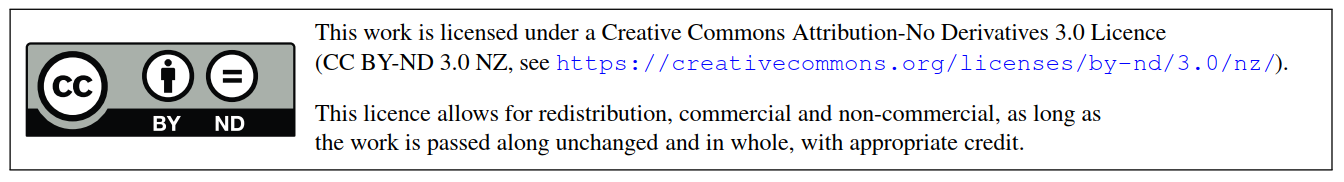
\includegraphics[scale=.41]{pictures/cc_license}
\end{center}

When using LaTeX, there is a Creative Commons license included in the style files for MSL Technical Guides and company reports.